\chapter{Results}

% analytical results
% * CPU tests for week run
% * Memory usage
% * speed comparisons w/ modes

\section{Stress Tests}

When we started developing BWLE we were aware of experiments running on ALE
spawning entire days \citep{mnih2015human}. Because of the huge amount of steps
steps required to learning policies based on some deep architecture, we decided
it was worth run a few stress-tests. We ran two experiments on the development
machine that lasting 5 days each.

The first experiment consisted in having a basic agent send random actions to
one unit for 5 million steps. We used the synchronous communication system and
fixed the observation-action rate per minute to 600 (10 Hz), ordering the client
to restart the game every 10000 iterations. The map consisted in an empty plane
with one unkillable controllable unit and one unkillable aggressive enemy unit
(as to force the game to do at least some planning all the time). The second
experiment followed the same procedure but stressed the game and BWAPI a bit
more heavily by including into the game an unusual number of in-game event
triggers and 100 units (split into 50 allied and 50 enemy units).

\begin{figure}[h]
    \centering
    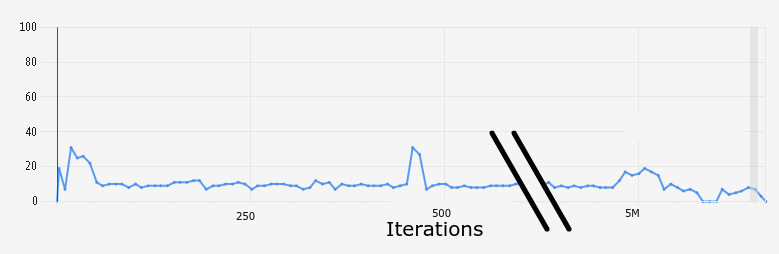
\includegraphics[width=\textwidth]{ch5/cpu_test_re}
    \caption{CPU usage of BWLE with respect to the Windows client and the Linux
      server. All the usage and was synchronously recorded every 10 steps. The
      memory usage closely follows the CPU usage.}
    \label{fig:fst_usage}
\end{figure}

The recorded usage (Figure \ref{fig:fst_usage}) shows a completely stable system
that can deal with both simple and complex maps using relatively few
computational resources. We did not achieve 100\% of branch coverage because we
didn't allow the usage of all the available actions, but the majority of the
client available interface was called at least once (according to Visual Studio
2013, 90\% of branch coverage was reached).

% TODO ADD NETWORK STATS

It must also be noted that most StarCraft AI tournaments \citep{...} run
BWAPI-based clients for entire weeks without any noticeable problem, so the
results we obtained were not unexpected.

\section{Navigation Task}

Next we tested our algorithms on the first StarCraft task, the``Navigation
Task''. The obtained results mostly matched our expectations: the task consisted
essentially in a medium-size grid-world which both algorithms managed to
eventually converge. Figure \ref{fig:nav_task_results} shows the average reward
per episode, where an episode is defined as the sequence of steps from the
starting state to a terminal state. The policies were evaluated every 10000
iterations by playing 10 episodes, recording mean and standard deviation.

\begin{figure}[h]
    \centering
    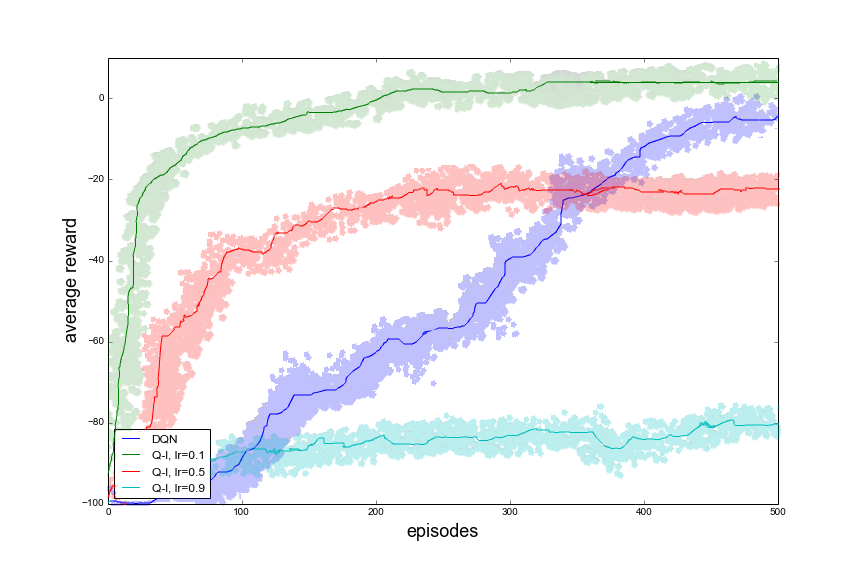
\includegraphics[width=\textwidth]{ch5/nav_task_re}
    \caption{Results of DQN and Q-learning on the simpler navigation task.}
    \label{fig:nav_task_results}
\end{figure}

Q-learning was tested with three different learning rates, while DQN was tested
using the same parameters used in \cite{mnih2015human}. We tried to do a more
appropriate sweep in the parameters space, but DQN tended to diverge when
varying too much some of the parameters and it would have taken too much time to
proceed with additional testing. Changing the action persistence window size
significantly impacted the learning process, as small windows made movement
actions too quick for the agent to switch from one block of the grid to the
other, rendering the task partially observable. We know that while DQN is stable
for MDPs, states with imperfect information in general require some stochastic
strategies to reach policies that are close to being optimal
\citep{heinrich2016deep}.

\section{Guided Navigation Task}

The experimental setting was similar to the previous experiment, beside having a
different map and reward function. DQN was trained using all the 20 available
maps, while Q-learning had to learn exclusively one map. This choice was made to
avoid having to find the correct parameters values, as the map was much larger
and we couldn't feasibly decrease the resolution of the grid without changing
the map's walkable paths average width.

\begin{figure}[h]
    \centering
    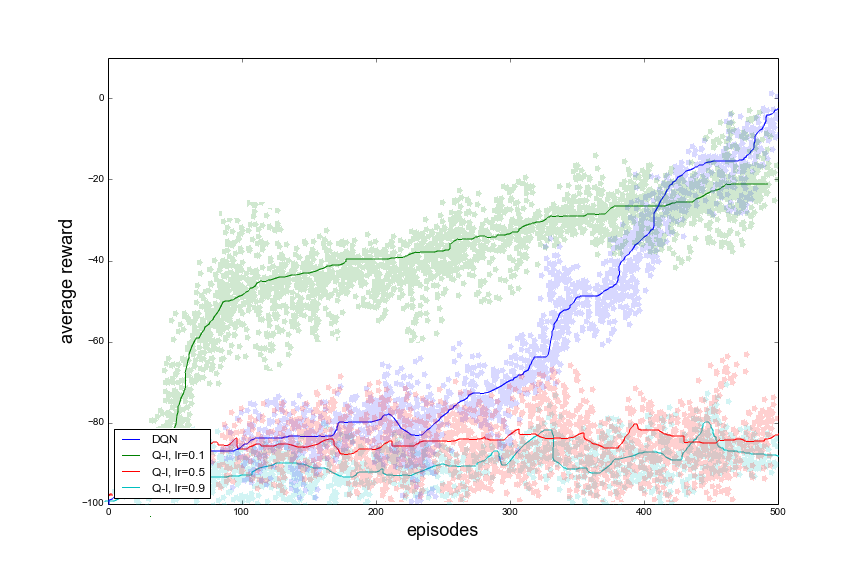
\includegraphics[width=\textwidth]{ch5/guid_task_re}
    \caption{Results of DQN and Q-learning on the guided navigation task.}
    \label{fig:guid_task_results}
\end{figure}

Figure \ref{fig:guid_task_results} shows the learning curve similarly to the
previous experiments. We can see that after a 200000 iterations the reward
starts to converge. 

\section{Survival Task}

Our last experimental setting was also the hardest. We hypothesised that both
algorithms would learn to survive by fighting, but we also expected the CNN to
acquire policies invariant to the units positions and more correlated to the
amount of units. We also expected to see more variance at evaluation time due to
the uneven difficulty of the designed maps.

% TODO Write the need to remove outliers.

Figure \ref{fig:surv_task_results} shows the results obtained by running
multi-unit Q-learning and multi-unit DQN. As predicted, the standard deviation
of the episodic reward arrays ended up being much higher compared to the other
tasks because some of the maps were significantly harder than others (as some
units were doomed to die). We can see that the average amount of steps in an
episode gradually increases, which means that learning is happening.

\begin{figure}[h]
    \centering
    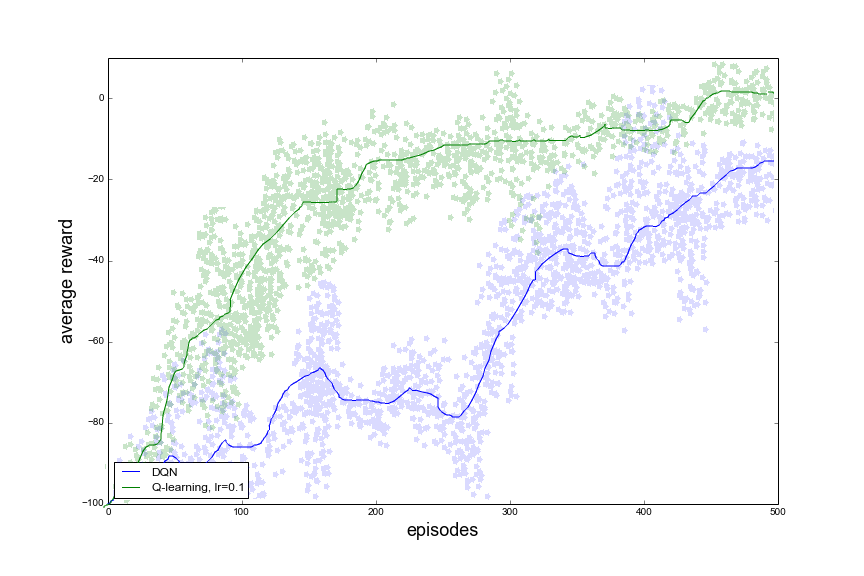
\includegraphics[width=\textwidth]{ch5/surv_task_re}
    \caption{Results of DQN and Q-learning on the harder Survival task.}
    \label{fig:surv_task_results}
\end{figure}

If we look at Figure \ref{fig:dif_pol} we can see that the distribution of
actions taken by each unit differs significantly depending on the amount of
allied and enemy units. It's interesting to note that there is some difference
between the policy learnt by the mono-unit agent and the one learnt by the
multi-unit version in the case when identical states are presented (for instance
0 allied units), but this is probably due to approximation noise in the
value network.

% simple tests
%  message checks
%  image checks
%  screen movement policy
%  grid movement
% many vs one unit

% multi-unit setting
% change of action window
% easy maps vs hard maps

\section{Chapter Summary}

In this chapter we presented the results of the experiments described in Chapter
4. We confirmed some of our initial hypotheses and tested the platform to its
limits, providing a baseline for future design and research work.
